% Options for packages loaded elsewhere
\PassOptionsToPackage{unicode}{hyperref}
\PassOptionsToPackage{hyphens}{url}
%
%\documentclass[
%]{book}
\documentclass[landscape, 20pt]{extreport}

\usepackage{amsmath,amssymb}
\usepackage{lmodern}
\usepackage{iftex}
\ifPDFTeX
  \usepackage[T1]{fontenc}
  \usepackage[utf8]{inputenc}
  \usepackage{textcomp} % provide euro and other symbols
\else % if luatex or xetex
  \usepackage{unicode-math}
  \defaultfontfeatures{Scale=MatchLowercase}
  \defaultfontfeatures[\rmfamily]{Ligatures=TeX,Scale=1}
\fi
% Use upquote if available, for straight quotes in verbatim environments
\IfFileExists{upquote.sty}{\usepackage{upquote}}{}
\IfFileExists{microtype.sty}{% use microtype if available
  \usepackage[]{microtype}
  \UseMicrotypeSet[protrusion]{basicmath} % disable protrusion for tt fonts
}{}
\makeatletter
\@ifundefined{KOMAClassName}{% if non-KOMA class
  \IfFileExists{parskip.sty}{%
    \usepackage{parskip}
  }{% else
    \setlength{\parindent}{0pt}
    \setlength{\parskip}{6pt plus 2pt minus 1pt}}
}{% if KOMA class
  \KOMAoptions{parskip=half}}
\makeatother
\usepackage{xcolor}
\IfFileExists{xurl.sty}{\usepackage{xurl}}{} % add URL line breaks if available
\IfFileExists{bookmark.sty}{\usepackage{bookmark}}{\usepackage{hyperref}}
\hypersetup{
  pdftitle={SCMA 470 : Risk Analysis and Credibility Tutorial 3},
  pdfauthor={Pairote Satiracoo},
  hidelinks,
  pdfcreator={LaTeX via pandoc}}
\urlstyle{same} % disable monospaced font for URLs
\usepackage[margin=1in]{geometry}
\usepackage{color}
\usepackage{fancyvrb}
\newcommand{\VerbBar}{|}
\newcommand{\VERB}{\Verb[commandchars=\\\{\}]}
\DefineVerbatimEnvironment{Highlighting}{Verbatim}{commandchars=\\\{\}}
% Add ',fontsize=\small' for more characters per line
\usepackage{framed}
\definecolor{shadecolor}{RGB}{248,248,248}
\newenvironment{Shaded}{\begin{snugshade}}{\end{snugshade}}
\newcommand{\AlertTok}[1]{\textcolor[rgb]{0.94,0.16,0.16}{#1}}
\newcommand{\AnnotationTok}[1]{\textcolor[rgb]{0.56,0.35,0.01}{\textbf{\textit{#1}}}}
\newcommand{\AttributeTok}[1]{\textcolor[rgb]{0.77,0.63,0.00}{#1}}
\newcommand{\BaseNTok}[1]{\textcolor[rgb]{0.00,0.00,0.81}{#1}}
\newcommand{\BuiltInTok}[1]{#1}
\newcommand{\CharTok}[1]{\textcolor[rgb]{0.31,0.60,0.02}{#1}}
\newcommand{\CommentTok}[1]{\textcolor[rgb]{0.56,0.35,0.01}{\textit{#1}}}
\newcommand{\CommentVarTok}[1]{\textcolor[rgb]{0.56,0.35,0.01}{\textbf{\textit{#1}}}}
\newcommand{\ConstantTok}[1]{\textcolor[rgb]{0.00,0.00,0.00}{#1}}
\newcommand{\ControlFlowTok}[1]{\textcolor[rgb]{0.13,0.29,0.53}{\textbf{#1}}}
\newcommand{\DataTypeTok}[1]{\textcolor[rgb]{0.13,0.29,0.53}{#1}}
\newcommand{\DecValTok}[1]{\textcolor[rgb]{0.00,0.00,0.81}{#1}}
\newcommand{\DocumentationTok}[1]{\textcolor[rgb]{0.56,0.35,0.01}{\textbf{\textit{#1}}}}
\newcommand{\ErrorTok}[1]{\textcolor[rgb]{0.64,0.00,0.00}{\textbf{#1}}}
\newcommand{\ExtensionTok}[1]{#1}
\newcommand{\FloatTok}[1]{\textcolor[rgb]{0.00,0.00,0.81}{#1}}
\newcommand{\FunctionTok}[1]{\textcolor[rgb]{0.00,0.00,0.00}{#1}}
\newcommand{\ImportTok}[1]{#1}
\newcommand{\InformationTok}[1]{\textcolor[rgb]{0.56,0.35,0.01}{\textbf{\textit{#1}}}}
\newcommand{\KeywordTok}[1]{\textcolor[rgb]{0.13,0.29,0.53}{\textbf{#1}}}
\newcommand{\NormalTok}[1]{#1}
\newcommand{\OperatorTok}[1]{\textcolor[rgb]{0.81,0.36,0.00}{\textbf{#1}}}
\newcommand{\OtherTok}[1]{\textcolor[rgb]{0.56,0.35,0.01}{#1}}
\newcommand{\PreprocessorTok}[1]{\textcolor[rgb]{0.56,0.35,0.01}{\textit{#1}}}
\newcommand{\RegionMarkerTok}[1]{#1}
\newcommand{\SpecialCharTok}[1]{\textcolor[rgb]{0.00,0.00,0.00}{#1}}
\newcommand{\SpecialStringTok}[1]{\textcolor[rgb]{0.31,0.60,0.02}{#1}}
\newcommand{\StringTok}[1]{\textcolor[rgb]{0.31,0.60,0.02}{#1}}
\newcommand{\VariableTok}[1]{\textcolor[rgb]{0.00,0.00,0.00}{#1}}
\newcommand{\VerbatimStringTok}[1]{\textcolor[rgb]{0.31,0.60,0.02}{#1}}
\newcommand{\WarningTok}[1]{\textcolor[rgb]{0.56,0.35,0.01}{\textbf{\textit{#1}}}}
\usepackage{longtable,booktabs,array}
\usepackage{calc} % for calculating minipage widths
% Correct order of tables after \paragraph or \subparagraph
\usepackage{etoolbox}
\makeatletter
\patchcmd\longtable{\par}{\if@noskipsec\mbox{}\fi\par}{}{}
\makeatother
% Allow footnotes in longtable head/foot
\IfFileExists{footnotehyper.sty}{\usepackage{footnotehyper}}{\usepackage{footnote}}
\makesavenoteenv{longtable}
\usepackage{graphicx}
\makeatletter
\def\maxwidth{\ifdim\Gin@nat@width>\linewidth\linewidth\else\Gin@nat@width\fi}
\def\maxheight{\ifdim\Gin@nat@height>\textheight\textheight\else\Gin@nat@height\fi}
\makeatother
% Scale images if necessary, so that they will not overflow the page
% margins by default, and it is still possible to overwrite the defaults
% using explicit options in \includegraphics[width, height, ...]{}
\setkeys{Gin}{width=\maxwidth,height=\maxheight,keepaspectratio}
% Set default figure placement to htbp
\makeatletter
\def\fps@figure{htbp}
\makeatother
\setlength{\emergencystretch}{3em} % prevent overfull lines
\providecommand{\tightlist}{%
  \setlength{\itemsep}{0pt}\setlength{\parskip}{0pt}}
\setcounter{secnumdepth}{5}
\usepackage{booktabs}
\usepackage{amsthm}
\usepackage{LectureNoteMacro}
\usepackage{bbm}
\usepackage{mathtools}
\makeatletter
\def\thm@space@setup{%
  \thm@preskip=8pt plus 2pt minus 4pt
  \thm@postskip=\thm@preskip
}
\makeatother
\ifLuaTeX
  \usepackage{selnolig}  % disable illegal ligatures
\fi
\usepackage[]{natbib}
\bibliographystyle{apalike}

\title{\textbf{SCMA 470 : Risk Analysis and Credibility} \textbf{Tutorial 3}}
\author{Pairote Satiracoo}
\date{2021-09-23}

\usepackage{amsthm}
\newtheorem{theorem}{Theorem}[chapter]
\newtheorem{lemma}{Lemma}[chapter]
\newtheorem{corollary}{Corollary}[chapter]
\newtheorem{proposition}{Proposition}[chapter]
\newtheorem{conjecture}{Conjecture}[chapter]
\theoremstyle{definition}
\newtheorem{definition}{Definition}[chapter]
\theoremstyle{definition}
\newtheorem{example}{Example}[chapter]
\theoremstyle{definition}
\newtheorem{exercise}{Exercise}[chapter]
\theoremstyle{definition}
\newtheorem{hypothesis}{Hypothesis}[chapter]
\theoremstyle{remark}
\newtheorem*{remark}{Remark}
\newtheorem*{solution}{Solution}
\begin{document}
\maketitle


\hypertarget{collective-risk-model}{%
\chapter{Collective Risk Model}\label{collective-risk-model}}

Mathematical models of the total amount of claims from a portfolio of
policies over a short period of time will be presented in this chapter.
The models are referred to as short term risk models. Two main sources
of uncertainty including the claim numbers and claim sizes will be taken
into consideration. We will begin with the model for aggregate (total)
claims or collective risk models.

We define the following random variables:

\begin{itemize}
\item
  \(S\) denotes total amount of claims from a portfolio of policies in a
  fixed time interval, for e.g.~one year,
\item
  \(N\) represents the number of claims, and
\item
  \(X_i\) denotes the amount of the \(i\)th claim.
\end{itemize}

Then the total claims \(S\) is given by \[S = X_1 + \ldots + X_N.\]

The following assumptions are made for deriving the collective risk
model:

\begin{enumerate}
\def\labelenumi{\arabic{enumi}.}
\item
  \(\{X_i \}_{i=1}^\infty\) are independent and identically distributed
  with distribution function \(F_X\).
\item
  \(N\) is independent of \(\{X_i \}_{i=1}^\infty\).
\end{enumerate}

The distribution of the total claim \(S\) is said to be a compound
distribution. The properties of the compound distribution will be given
in the Section \protect\hyperlink{sectionCompoundDistribution}{2}.

\textbf{Note} The distribution of \(S\) can be derived by using convolution
technique. In general, the closed form expressions for the compound
distribution do not exist so we will mainly concern with the moments of
\(S\). For more details about convolution, see Gray and Pitts (2012).

\hypertarget{conditional-expectation-and-variance-formulas}{%
\section{Conditional expectation and variance formulas}\label{conditional-expectation-and-variance-formulas}}

Some useful properties of conditional expectation and conditional
variance are given. The conditional expectaion formula is

\[E[ E[X|Y ]] = E[X].\] The conditional variance of \(X\) given \(Y\) is
defined to be
\[\begin{split}
    Var[X|Y]   &= Var[Z] \text{ where } Z = X|Y  \\
            &= E[(Z - E[Z])^2] = E[Z^2] - (E[Z])^2 \\
            &= E[(X - E[X|Y])^2  | Y] \\
            &= E[X^2| Y] - (E[X|Y])^2. \\
\end{split}\]
The conditional variance formula is
\begin{equation} 
\label{eq:exampleVariance}
    Var[X] = E[ Var[X|Y ]] + Var[E[X|Y ]].
\end{equation}

\begin{example}
\protect\hypertarget{exm:unlabeled-div-39}{}\label{exm:unlabeled-div-39}

Show that \[Var[X] = E[ Var[X|Y ]] + Var[E[X|Y ]].\]

\end{example}

\textbf{Solution:}

Consider the terms on the right-hand side of \eqref{eq:exampleVariance}. We have

\[\begin{aligned}
    E[Var[X|Y]] &= E\left[  E[X^2|Y] -  (E[X|Y])^2   \right] \\
        &=  E[X^2] - E\left[(E[X|Y])^2   \right],
    \end{aligned}\] and
\[\begin{aligned}
    Var[E[X|Y ]]  &= Var[Z] \text{ where } Z = E[X|Y ]  \\
                &= E[(E[X|Y ])^2] - (E[E[X|Y ]])^2 \\
                &= E[(E[X|Y ])^2] - (E[X])^2 \\
                \end{aligned}\] Adding
both terms gives the required result.

\begin{example}
\protect\hypertarget{exm:unlabeled-div-40}{}\label{exm:unlabeled-div-40}

In three coloured boxes - Red, Green and Blue, each box has two bags.
The bags of Red box contain 1 and 2 (in units of THB) respectively, those of Green box contain
1 and 5, and those of Blue contain 1 and 10 . A box is chosen at random in such
a way that
\(\Pr(\text{Red}) = \Pr(\text{Green}) = \Pr(\text{Blue}) = 1/3\). A fair
coin is tossed to determined which bag to be chosen from the chosen box.
Let \(X\) be the value of the contents of the chosen bag.

\begin{enumerate}
\def\labelenumi{\arabic{enumi}.}
\item
  Find the distribution of \(X\).
\item
  Find \(E[X]\) and \(Var[X]\).
\item
  Use the conditional expectation and conditional variance formulas to
  verify your results.
\end{enumerate}

\end{example}

\textbf{Solution:}
1. The distribution of \(X\) can be obtained by using the law of total
probability: for example \[\begin{aligned}
        P(X= 1) &= P(X = 1 , R) + P(X = 1 , G) + P(X = 1 , B) \\ 
        &= P(X = 1 | R) \cdot P(R) + P(X = 1 | G) \cdot P(G) + P(X = 1 | B) \cdot P(B) \\
        &= \frac{1}{2} \cdot  \frac{1}{3} + \frac{1}{2} \cdot  \frac{1}{3} + \frac{1}{2} \cdot  \frac{1}{3} = \frac{1}{2}.
        \end{aligned}\]
Similarly, we have
\[P(X = 1 ) = \frac{1}{2}, \quad P(X = 2 ) =  P(X = 5 ) =  P(X = 10 ) =  \frac{1}{6}.\]

\begin{enumerate}
\def\labelenumi{\arabic{enumi}.}
\setcounter{enumi}{1}
\item
  It follows that
  \[E[X] = \frac{10}{3}, \quad Var[X] = \frac{98}{9}.\]
\item
  We first calculate \[\begin{aligned}
      E[X|R] &= \frac{1}{2}\cdot(1 + 2) = \frac{3}{2} \\
      E[X|G] &= \frac{1}{2}\cdot(1 + 5) = 3 \\
      E[X|B] &= \frac{1}{2}\cdot(1 + 10) = \frac{11}{2}. \\  \end{aligned}\]
  We have \[\begin{aligned}
      E[X] &= E[X | R] \cdot P(R) + E[X | G] \cdot P(G)  + E[X | B] \cdot P(B)  \\
      &= \frac{1}{3}\cdot(\frac{3}{2}  + 3 + \frac{11}{2}) = \frac{10}{3}.  \end{aligned}\]
\end{enumerate}

\hypertarget{sectionCompoundDistribution}{%
\section{\texorpdfstring{The moments of a compound distribution \(S\)}{The moments of a compound distribution S}}\label{sectionCompoundDistribution}}

The moments and moment generating function of \(S\) can be easily derived
from the conditional expectation formula.

\hypertarget{the-mean-of-s}{%
\subsection{\texorpdfstring{The mean of \(S\)}{The mean of S}}\label{the-mean-of-s}}

Let \(m_k\) be the \(k\)th moment of \(X_1\), i.e.~\(E[X_1^k] = m_k\).
Conditional on \(N = n\), we have
\[E[S | N = n] = E[ \sum_{i=1}^n X_i] = \sum_{i=1}^n E[ X_i] = n E[ X_i] = n \cdot m_1.\]
Hence, \(E[S | N] = N m_1\) and
\[E[S] =   E[E[S | N]] = E[N m_1] = E[N] m_1 = E[N] \cdot E[X_1].\]
It is no surprise that the mean of the total claims is the product of
the means of the number of claims and the mean of claim sizes.

\hypertarget{the-variance-of-s}{%
\subsection{\texorpdfstring{The variance of \(S\)}{The variance of S}}\label{the-variance-of-s}}

Using the fact that \(\{X_i \}_{i=1}^\infty\) are independent, we have
\[Var[S | N = n] = Var[ \sum_{i=1}^n X_i] = \sum_{i=1}^n Var[ X_i] = n Var[ X_i]  =n (m_2 - m_1^2),\]
and \(Var[S | N] = N (m_2 - m_1^2).\) It follows that \[\begin{aligned}
    Var[S] &= E[ Var[S | N] ] + Var[ E[S | N] ] \\
           &= E[ N (m_2 - m_1^2) ] + Var[ N m_1 ] \\
           &= E[ N ]  (m_2 - m_1^2)  +  Var[ N ] m_1  ^2. \end{aligned}\]

\begin{example}
\protect\hypertarget{exm:unlabeled-div-41}{}\label{exm:unlabeled-div-41}

Show that \(M_S(t) = M_N(\log(M_X(t)))\).

\end{example}

\textbf{Solution:}

First, consider the following conditional expectation: \[\begin{aligned}
    E\left [e^{t S} | N = n \right] &= E\left[e^{t (X_1 + X_2 + \cdots X_n)}\right] \\
                 &= E\left[e^{t X_1}\right]  \cdot E\left[e^{t X_2}\right]  \cdots E\left[e^{t X_n}\right]  \text{, since } X_1, X_2 \ldots, X_n \text{ are independent} \\ 
                 &= (M_X(t))^n.\end{aligned}\] Hence
\(E \left [e^{t S} | N \right] = (M_X(t))^N.\)

From the definition of the moment generating function, \[\begin{aligned}
    M_S(t) &= E[e^{t S}] \\
        &= E \left[  E[e^{t S} | N] \right ] \\
        &= E \left[ (M_X(t))^N  \right ]\\
        &= E \left[  Exp( N \cdot \log (M_X(t) )    \right] \\
        &= M_N(\log(M_X(t)))   (\text{ since } M_X(t) = E[e^{tX}] ).\end{aligned}\]

\hypertarget{special-compound-distributions}{%
\section{Special compound distributions}\label{special-compound-distributions}}

\hypertarget{compound-poisson-distributions}{%
\subsection{Compound Poisson distributions}\label{compound-poisson-distributions}}

Let \(N\) be a Poisson distribution with the parameter \(\lambda\), i.e.
\(N \sim Poisson(\lambda)\) and \(\{X_i \}_{i=1}^\infty\) are independent and
identically distributed with distribution function \(F_X\). Then
\(S = X_1 + \ldots + X_N\) is said to have a compound Poisson distribution
and denote by \(\mathcal{CP}(\lambda,F_X)\).

\textbf{Note} The same terminology can be defined similarly for other
distributions, for e.g.~if \(N\) has a negative binomial distribution,
then \(S\) is said to have a compound negative binomial distribution.

\begin{example}
\protect\hypertarget{exm:unlabeled-div-42}{}\label{exm:unlabeled-div-42}

Let \(S \sim \mathcal{CP}(\lambda,F_X)\). Show that

\begin{enumerate}
\def\labelenumi{\arabic{enumi}.}
\item
  \(E[S] = \lambda m_1\),
\item
  \(Var[S] = \lambda m_2\),
\item
  \(M_S(t) = Exp{(\lambda(M_X(t) - 1))}.\)
\item
  The third central moment \(E[(S- E[S])^3] = \lambda m_3\), and hence
  \[Sk[S] = \frac{\lambda m_3}{(\lambda m_2)^{3/2}},\]
\end{enumerate}

where \(m_k\) be the \(k\)th moment of \(X_1\)

\end{example}

\textbf{Solution:}
1. \(E[S] = E[N] \cdot E[X] = \lambda m_1\),

\begin{enumerate}
\def\labelenumi{\arabic{enumi}.}
\setcounter{enumi}{1}
\item
  \(Var[S] = E[ N ] (m_2 - m_1^2) + Var[ N ] m_1 ^2 =  \lambda(m_2 - m_1^2) + \lambda m_1^2 = \lambda m_2\),
\item
  From \[\begin{aligned}
          M_S(t) &=  M_N(\log(M_X(t))) \\
              &= Exp\left( \lambda  \left( e^{\log(M_X(t))} - 1   \right)  \right), \text{ since } M_N(t) = Exp(\lambda(e^t - 1))  \\
              &= Exp{(\lambda(M_X(t) - 1))}.
      \end{aligned}\]
\item
  The third central moment \(E[(S- E[S])^3] = \lambda m_3\), and hence
  \[Sk[S] = \frac{\lambda m_3}{(\lambda m_2)^{3/2}}.\] In particular,
  we have \[\begin{aligned}
      E[(N- E[N])^3] &= E\left [  N^3 - 3 N^2  \cdot E[N] + 3 N \cdot  (E[N])^2 - (E[N])^3       \right]  \\
          &= E[N^3] - 3 E[N^2]  \cdot E[N] + 2 (E[N])^3 \\
          &= M_N'''(0) - 3  M_N''(0) \cdot  M_N'(0) + 2 (M_N'(0))^3\end{aligned}\]

  For \(N \sim Poisson(\lambda)\), \(M_N(t) = Exp(\lambda(e^t - 1)).\) By
  differentiating \(M_N(t)\) and evaluating at \(t = 0\), we can show that
  \[M'(0) = \lambda, \quad  M''(0) = \lambda (1 + \lambda), \quad M'''(0) = \lambda (1 + 3\lambda + \lambda^2).\]
  Hence, \(E[(N- E[N])^3] = \lambda.\)

  Similarly,

  \[\begin{aligned}
      E[(S- E[S])^3] &=  E[S^3] - 3 E[S^2]  \cdot E[S] + 2 (E[S])^3 \\
    \end{aligned}\]
  In addition, \(M_S(t) = Exp{(\lambda(M_X(t) - 1))}.\) By
  differentiating \(M_S(t)\) we can show that \[\begin{aligned}
      M'''_S(t) &= \lambda M'''_X(t) M_S(t)   + 2 \lambda M''_X(t) M'_S(t)  + \lambda M'_X(t) M''_S(t).\\ \end{aligned}\]
  Evaluating \(M'''_S(t)\) at \(t = 0\) results in \[\begin{aligned}
      M'''_S(0) &= E[S^3] = \lambda m_3 + 3 E[S] \cdot E[S^2] - 2( E[S])^3,\end{aligned}\]
  which gives \[\begin{aligned}
      E[(S- E[S])^3] &=  E[S^3] - 3 E[S^2]  \cdot E[S] + 2 (E[S])^3 \\
          &= \lambda m_3.\end{aligned}\]
\end{enumerate}

\begin{example}
\protect\hypertarget{exm:unlabeled-div-43}{}\label{exm:unlabeled-div-43}

Let \(S\) be the aggregate annual claims for a risk where
\(S \sim \mathcal{CP}(10,F_X)\) and the individual claim amounts have a
\(Pa(4,1)\) distribution. Calculate \(E[S], Var[S]\) and \(Sk[S]\).

\end{example}

\textbf{Solution:}
Since \(X \sim Pa(4,1)\) with \(\alpha = 4\) and \(\lambda = 1\), we
have \[\begin{aligned}
E[X^r] &= \frac{\Gamma(\alpha - r) \cdot \Gamma(1 + r) \cdot \lambda^r  }{\Gamma(\alpha)}\\
E[X] &= \frac{\lambda}{\alpha - 1} = \frac{1}{4-1} = \frac{1}{3}\\
E[X^2] &=  \frac{\Gamma(2) \cdot \Gamma(3) \cdot \lambda^2  }{\Gamma(4)} = \frac{1}{3}\\ 
E[X^3] &=  \frac{\Gamma(1) \cdot \Gamma(4) \cdot \lambda^3  }{\Gamma(4)} = 1.\\ \end{aligned}\]
We have \[\begin{aligned}
E[S]  &= \lambda E[X] = \frac{10}{3} \\
Var[S] &= \lambda E[X^2] = \frac{10}{3} \\
Sk[S] &= \frac{\lambda E[X^3]}{\left(\lambda E[X^2]\right)^{3/2}} = \frac{10}{(10/3)^{3/2}} = 1.6432.\\ \end{aligned}\]\\

In what follows, we will use R to simulate \(n\) observations from a compound Poisson distribution, where the Poisson parameter is \(\lambda\) and where the claims are exponentially distributed with mean \(\mu\), i.e.~
\(CP(\lambda, Exp(1/\mu))\)

\begin{Shaded}
\begin{Highlighting}[]
\CommentTok{\# Simulation n observations from a  CP(lambda,FX) distribution}
\CommentTok{\# Assumptions:}
\CommentTok{\# N \textasciitilde{} Poisson(lambad)}
\CommentTok{\# X \textasciitilde{} Pa(alpha,beta)}
\FunctionTok{library}\NormalTok{(actuar)}

\NormalTok{n }\OtherTok{\textless{}{-}} \DecValTok{10000}
\NormalTok{lambda }\OtherTok{\textless{}{-}}  \DecValTok{10}
\NormalTok{alpha }\OtherTok{\textless{}{-}} \DecValTok{4}
\NormalTok{beta }\OtherTok{\textless{}{-}} \DecValTok{1}

\NormalTok{totalClaims }\OtherTok{\textless{}{-}} \FunctionTok{rep}\NormalTok{(}\DecValTok{0}\NormalTok{,n)}
\NormalTok{numclaims }\OtherTok{\textless{}{-}} \FunctionTok{rpois}\NormalTok{(n,lambda)}
\ControlFlowTok{for}\NormalTok{ (i }\ControlFlowTok{in} \DecValTok{1}\SpecialCharTok{:}\NormalTok{n)}
\NormalTok{  totalClaims[i] }\OtherTok{\textless{}{-}} \FunctionTok{sum}\NormalTok{(}\FunctionTok{rpareto}\NormalTok{(numclaims[i], }\AttributeTok{shape =}\NormalTok{alpha, }\AttributeTok{scale =}\NormalTok{ beta))}
\FunctionTok{hist}\NormalTok{(totalClaims)}
\end{Highlighting}
\end{Shaded}

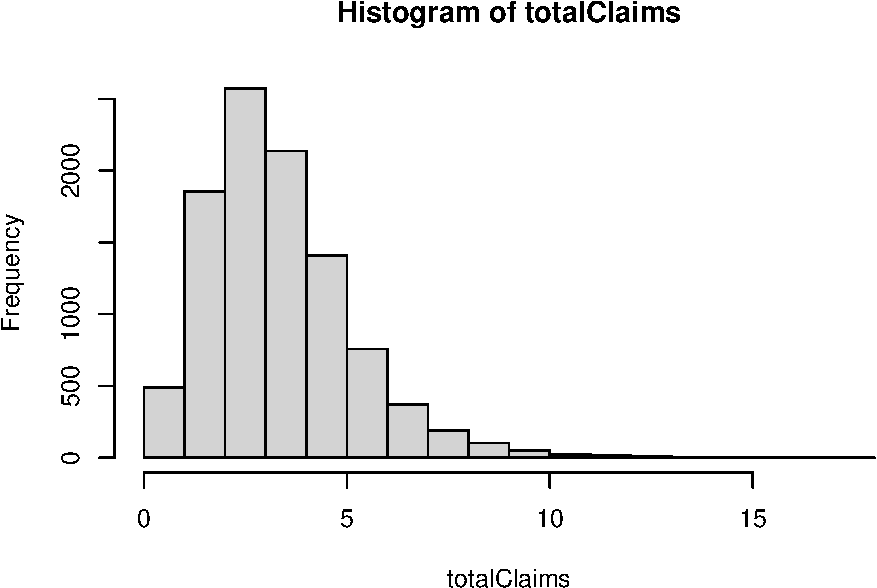
\includegraphics{simulationCP-1.pdf}

\begin{Shaded}
\begin{Highlighting}[]
\FunctionTok{mean}\NormalTok{(totalClaims)}
\end{Highlighting}
\end{Shaded}

\begin{verbatim}
## [1] 3.338976
\end{verbatim}

\begin{Shaded}
\begin{Highlighting}[]
\FunctionTok{var}\NormalTok{(totalClaims)}
\end{Highlighting}
\end{Shaded}

\begin{verbatim}
## [1] 3.29011
\end{verbatim}

\begin{Shaded}
\begin{Highlighting}[]
\FunctionTok{library}\NormalTok{(moments)}
\FunctionTok{skewness}\NormalTok{(totalClaims)}
\end{Highlighting}
\end{Shaded}

\begin{verbatim}
## [1] 1.345385
\end{verbatim}

\textbf{Note}
An important property of independent, but not necessarily identically
distributed, compound Poisson random variables is that the sum of a
fixed number of them is also a compound Poisson random variable.

\begin{example}
\protect\hypertarget{exm:Additivity}{}\label{exm:Additivity}

Let \(S_1, \ldots, S_n\)
be independent compound Poisson random variables, with parameters
\(\lambda_i\) and \(F_i\). Then \(S = \sum_{i=1}^n S_i\) has a compound
distribution with parameter \[\lambda =  \sum_{i=1}^n \lambda_i,\] and
\[F = \frac{1}{\lambda}\sum_{i=1}^n \lambda_i F_i.\]

\end{example}

\textbf{Solution:}
Exercise.

\textbf{Note} The compound Poisson distribution is the most often used in
practice. It possesses the additivity of independent compound Poisson
distributions (as shown in
Example \ref{exm:Additivity}, and the expressions of the first three moments
are very simple.

\hypertarget{compound-negative-binomial-distributions}{%
\subsection{Compound negative binomial distributions}\label{compound-negative-binomial-distributions}}

A useful discrete random variable that can be used for modelling the
distributions of claim numbers is a negative binomial distribution. A
random variable \(N\) has a negative distribution with parameters \(k\) and
\(p\), denoted by \(N \sim NB(k,p)\) if its probability mass function is given
by
\[f_N(n) = \Pr(N = n) = \frac{\Gamma(k+n)}{\Gamma(n+1)\Gamma(k)} p^k (1- p)^n \quad n = 0,1,2,\ldots.\]
It can be interpreted as the probability of getting \(n\) failures before
the \(k\)th success occurs in a sequence of independent Bernoulli trials
with probability of success \(p\).

\begin{example}
\protect\hypertarget{exm:unlabeled-div-44}{}\label{exm:unlabeled-div-44}

Let \(N \sim NB(k,p)\). Show that the mean, variance and moment generating
function of the compound negative binomial distribution, denoted by
\(\mathcal{CNB}(k,p,F_X)\), are as follows:

\begin{enumerate}
\def\labelenumi{\arabic{enumi}.}
\item
  \(E[S] = \frac{k q}{p} m_1\),
\item
  \(Var[S] = \frac{k q}{p^2} (p m_2 + q m_1^2)\),
\item
  \(M_S(t) = \left( \frac{ p }{ 1 - q M_X(t) } \right)^k,\)
\end{enumerate}

where \(m_k\) be the \(k\)th moment of \(X_1\) and \(q = 1-p\).

\end{example}

\textbf{Solution:}
The results follows from the properties of the negative binomial
distribution \(N \sim NB(k,p)\):
\[E[N] = \frac{kq}{p}, \quad Var[N] = \frac{kq}{p^2},\] and the
moments of a compound distribution \(S\) derived in Section
\ref{sectionCompoundDistribution}.

\textbf{Notes}
1. The negative binomial distribution is an alternative to the Poisson distribution for \(N\), in the sense that it allows for any value of \(N = 0, 1, 2, \ldots\), unlike the binomial
distribution which has an upper limit.

One advantage that the negative binomial distribution has over the Poisson distribution is that its variance exceeds its mean. These two quantities are equal for the Poisson distribution.

Thus, the negative binomial distribution may give a better fit to a data set which has a sample variance in excess of the sample mean.

\begin{enumerate}
\def\labelenumi{\arabic{enumi}.}
\setcounter{enumi}{1}
\tightlist
\item
  The compound negative binomial distribution is an appropriate to model the heterogeneity of the numbers of claims occurring for
  different risks. In particular, suppose that for each policy, the number
  of claims in a year has a Poisson distribution
  \(N | \lambda \sim Poisson(\lambda)\), and that the variation in \(\lambda\) across
  the portfolio can be modelled using a Gamma distribution \(\mathcal{G}(\alpha, \lambda)\). Then
  the number of claims in the year for a policy chosen at random from the
  portfolio has a negative binomial distribution.
\end{enumerate}

\hypertarget{misture-distributions}{%
\subsubsection{Misture distributions}\label{misture-distributions}}

Suppose we model a policyholder's claim number \(N\) using a conditional distribution \(N | \lambda\), where \(\lambda\) can be thought of as a ``risk parameter'' for that policyholder.

Policyholders represent a variety of risks and have different risk parameters, and we model the variation across policyholders by regarding the various \(\lambda\)s as being independent realisations of a random variable with known probability distribution. This gives the joint density, which we can write as
\(f_{N,\lambda}(k, \lambda) = f_\lambda(\lambda) f_{N|\lambda}(k | \lambda)\).

This enables us to allow for variability in the risks across a portfolio; that is, to model the heterogeneity of the numbers of claims occurring for different risks.

\begin{example}
\protect\hypertarget{exm:unlabeled-div-45}{}\label{exm:unlabeled-div-45}

A portfolio consists of a large number of individual policies. For each policy, the number of claims in a year has a poisson distribution \(N | \lambda \sim Poisson(\lambda)\). Let us suppose that the variation in \(\lambda\) across the portfolio of risks can be modelled using a gamma \(\mathcal{G}(\alpha,\beta)\) distribution with known parameters, and let us use this to average across the risks.

We are considering a \textbf{mixture} of Poissons where the mixing distribution if gamma. This is also known as a mixture \textbf{distribution}. Derive the probability mass function of the mixture distribution.

\end{example}

\textbf{Solution:}

For \(k = 0,1,2,\ldots\), we have

\[
\begin{aligned}
\Pr(N = k) &= \int f_\lambda(\lambda) \Pr(N = k | \lambda) \, d\lambda \\
&= \int_{0}^\infty \frac{\beta^\alpha}{\Gamma(\alpha)} \lambda^{\alpha -1} e^{\beta \lambda} e^{-\lambda} \frac{\lambda^k}{k!} \, d\lambda \\
&= \frac{\Gamma(\alpha + k)}{\Gamma(\alpha) \Gamma(1 + k)} \frac{\beta^\alpha}{(\beta+1)^{\alpha+k}} \times \int_0^\infty h(\lambda) \, d\lambda 
\end{aligned}
\]
where \(h(\lambda)\) is the probability density function of \(\lambda \sim \mathcal{G}(\alpha + k, \beta + 1)\).

Hence,

\[ \Pr(N =k) = \frac{\Gamma(\alpha + k)}{\Gamma(\alpha) \Gamma(1 + k)} \left(\frac{\beta}{\beta+1}\right)^\alpha \left(\frac{1}{\beta+1}\right)^k, k = 0,1,2,\ldots,\]

which is the probability mass function of a \(\mathcal{NB}(\alpha, \beta/(\beta + 1))\) distribution.

This provides an illuminating view of the negative binomial distribution -- it arises as a mixture of Poissons where the mixing distribution is gamma.

\hypertarget{an-example-in-r}{%
\subsubsection{an Example in R}\label{an-example-in-r}}

This R Markdown introduces the concept of mixture distributions which applies to models for claim numbers.

Suppose we model a policyholder's claim numbers \(N\) using a conditional distribution \(N | \lambda\), where \(\lambda\) can be thought of as a \textbf{risk parameter} for that policyholder. Policyholders represent a variety of risks and have different risk parameters, and we model the variation across policyholders by regarding the various \(\lambda\)s as being independent realisations of a random variable with known probability distribution.

The following R code produces the required \(n\) simulated values from this mixture distribution, where \(N | \lambda \sim Poisson(\lambda)\) with mixing distribution \(\mathcal{G}(\alpha, \beta)\), i.e.~\(\lambda \sim \mathcal{G}(\alpha, \beta)\).

eyJsYW5ndWFnZSI6InIiLCJzYW1wbGUiOiJzZXQuc2VlZCg1MzUzKVxubiA8LSA1MDAwXG5hbHBoYSA8LSA0XG5iZXRhIDwtIDEvM1xubGFtYmRhIDwtIHJnYW1tYShuLCBzaGFwZSA9IGFscGhhLCByYXRlID0gYmV0YSlcbm51bWNsYWltcyA8LSBzYXBwbHkobGFtYmRhLHJwb2lzLG4gPTEpXG5oaXN0KG51bWNsYWltcylcbnByaW50KG1lYW4obnVtY2xhaW1zKSlcbnByaW50KHZhcihudW1jbGFpbXMpKVxuXG4jTWl4dHVyZSB+IG5iKGFscGhhLGJldGEvKGJldGErMSkpXG5hbHBoYU1peHR1cmUgPC0gYWxwaGFcbmJldGFNaXh0dXJlIDwtIGJldGEvKGJldGErMSlcbm1lYW5NaXh0dXJlIDwtIGFscGhhTWl4dHVyZSooMS1iZXRhTWl4dHVyZSkvYmV0YU1peHR1cmVcbnZhck1peHR1cmUgPC0gbWVhbk1peHR1cmUvYmV0YU1peHR1cmUifQ==

\hypertarget{compound-binomial-distributions}{%
\subsection{Compound binomial distributions}\label{compound-binomial-distributions}}

A compound binomial distribution can be used to model a portfolio of
policies, each of which can give rise to at most one claim.

\begin{example}
\protect\hypertarget{exm:unlabeled-div-46}{}\label{exm:unlabeled-div-46}

Consider a portfolio of \(n\) independent and identical policies where
there is at most one claim on each policy in a year (for e.g.~life
insurance). Let \(p\) be the probability that a claim occurs. Explain that
the aggregate sum \(S\) in this portfolio has a compound binomial
distribution, denoted by \(\mathcal{CB}(n,p,F_X)\). Derive the mean,
variance and moment generating function of \(S\).

\end{example}

\textbf{Solution:}
Since \(n\) policies (lives) are independent with the probability \(p\) that
a claim occurs, the number \(N\) of claims on the portfolio in one year
has a binomial distribution i.e.~\(N \sim \text{bi}(n,p)\). If the sizes
of the claims are i.i.d. random variables, independent of \(N\), then the
total amount \(S\) claimed on this policy in one year has a compound
binomial distribution.

The mean, variance and the moment generating function of \(S\) are as
follows: \[\begin{aligned}
E[S] &= n p m_1, \\
Var[S] &= np m_2 - n p^2 m_1^2, \\
M_S(t) &= \left( q + p  M_X(t)      \right)^n,\end{aligned}\] where
\(m_k\) be the \(k\)th moment of \(X_1\) and \(q = 1-p\).

\hypertarget{the-effect-of-reinsurance}{%
\section{The effect of reinsurance}\label{the-effect-of-reinsurance}}

The effect of reinsurance arrangements on an aggregate claims
distribution will be presented. Let \(S\) denotes the total aggregate
claims from a risk in a given time, \(S_I\) and \(S_R\) denote the insurance
and reinsurance aggregate claims, respectively. It follows that
\[S = S_I + S_R.\]

\hypertarget{proportional-reinsurance-1}{%
\subsection{Proportional reinsurance}\label{proportional-reinsurance-1}}

Recall that under proportional reinsurance arrangement, a fixed
proportion \(\alpha\) is paid by the direct insurer and the remainder of
the claim is paid by the reinsurer. It follows that
\[S_I =  \sum_{i= 1}^N  \alpha X_i = \alpha S\] and
\[S_R =  \sum_{i= 1}^N (1- \alpha) X_i = (1- \alpha) S,\] where \(X_i\) is
the amount of the \(i\)th claim.

\textbf{Notes}

\begin{enumerate}
\def\labelenumi{\arabic{enumi}.}
\item
  Both direct insurer and the reinsurer are involved in paying each
  claim.
\item
  Both have unlimited liability unless a cap on the claim amount is
  arranged.
\end{enumerate}

\begin{example}
\protect\hypertarget{exm:unlabeled-div-47}{}\label{exm:unlabeled-div-47}

Aggregate claims from a risk in a given time have a compound Poisson
distribution with Poisson parameter \(\lambda = 10\) and an individual
claim amount distribution that is a Pareto distribution,
\(Pa(4,1)\). The insurer has effected proportional reinsurance with
proportion retained \(\alpha = 0.8\).

\begin{enumerate}
\def\labelenumi{\arabic{enumi}.}
\item
  Find the distribution of \(S_I\) and \(S_R\) and their means and
  variances.
\item
  Compare the variances \(Var[S_I] +Var[S_R]\) and \(Var[S]\). Comment
  on the results obtained.
\end{enumerate}

\end{example}

\textbf{Solution:}
1. We have \[\begin{aligned}
    S_I &= \sum_{i=1}^N \left( \alpha X_i \right) = \alpha \sum_{i=1}^N X_i = \alpha \cdot S, \\
    S_R &= \sum_{i=1}^N \left( (1- \alpha) X_i \right) = (1- \alpha) \sum_{i=1}^N X_i = (1- \alpha) \cdot S,\end{aligned}\]
since both insurer and reinsurer are involved in paying each claim,
i.e.~\(Y_i = \alpha X_i\) and \(Z_i = (1- \alpha) X_i\). It follows that
\(S_I \sim \mathcal{CP}(10,F_Y)\) and \(S_R \sim \mathcal{CP}(10,F_Z)\).

\begin{enumerate}
\def\labelenumi{\arabic{enumi}.}
\setcounter{enumi}{1}
\item
  As we can show that if \(X \sim Pa(\beta,\lambda)\), then
  \(W = k X \sim Pa(\beta,k \lambda)\). For
  \(X \sim Pa(4,1)\) with \(\beta = 4\) and \(\lambda = 1\), we have
  \(Y_i \sim Pa(\beta, \alpha \cdot \lambda) = Pa(4, 0.8)\)
  and \[\begin{aligned}
  E[S_I] &= 10 \cdot E[Y_i] = 10   \cdot \frac{\alpha \cdot \lambda}{\beta - 1} \\
  & = \frac{8}{3}, \\
  Var[S_I] &=10 \cdot E[Y_i^2]  =   10 \cdot \frac{\Gamma(\beta - 2) \cdot \Gamma(1 + 2) \cdot (\alpha \cdot \lambda)^2  }{\Gamma(\beta)} \\
   &= 10 \cdot   \frac{\Gamma(2) \cdot \Gamma(3) \cdot (\alpha \cdot \lambda)^2  }{\Gamma(4)} = 10 \cdot \frac{2!}{3!} \cdot  (0.8)^2 \\
   &= \frac{32}{15} \end{aligned}\]

  Alternatively, we can calculate by using the properties of the
  expectation and variance as follows: \[\begin{aligned}
  E[S_I] &= E[\alpha S] = \alpha\cdot E[S] = \alpha\cdot \lambda \cdot E[X]  = 10 \cdot 0.8 \cdot \frac{1}{3} = \frac{8}{3}, \\
  Var[S_I] &= Var[\alpha S]  =  \alpha^2 \cdot Var[S] \\
         &= \alpha^2 \cdot \lambda \cdot E[X^2] = \frac{32}{15} .\end{aligned}\]
\end{enumerate}

Similarly, \[\begin{aligned}
E[S_R] &= E[(1 - \alpha) S] = (1 - \alpha)\cdot E[S] = \frac{2}{3}, \\
Var[S_R] &= Var[(1 - \alpha) S]  =  (1 - \alpha)^2 \cdot Var[S] =  \frac{2}{15} .\end{aligned}\]
Note that \(E[S_I] + E[S_R] = E[S]\), while
\(Var[S_I] + Var[S_R] = \frac{34}{15} < Var[S] = \frac{10}{3}.\)

\hypertarget{excess-of-loss-reinsurance-1}{%
\subsection{Excess of loss reinsurance}\label{excess-of-loss-reinsurance-1}}

Recall that under excess of loss reinsurance arrangement, the direct
insurer has effected excess of loss reinsurance with retention level
\(M >0\). For a claim \(X\),

\begin{itemize}
\item
  the insurance company pays any claim in full if \(X \le M\); and
\item
  the reinsurer (or reinsurance company) pays the remaining amount of
  \(X - M\) if \(X > M\).
\end{itemize}

It follows that

\begin{equation} 
\label{eq:eqnSI} S_I =  \sum_{i= 1}^N  Y_1 + Y_2 + \ldots + Y_N =  \sum_{i= 1}^N  \min(X_i,M)
\end{equation}
and
\begin{equation} 
\label{eq:eqnSR} S_R = \sum_{i= 1}^N  Z_1 + Z_2 + \ldots + Z_N  = \sum_{i= 1}^N \max(0,X_i - M), 
\end{equation}
where \(X_i\) is the amount of the \(i\)th claim.
When \(N = 0\), we set \(S_I = 0\) and \(S_R = 0\).

\textbf{Note} \(S_R\) can equal 0 even if \(N > 0\). This occurs when all claims
do not exceed \(M\) and hence the insurer pays the full amounts of claims.

As discussed in the previous section, the reinsurer is involved only
claims which exceed the retention limit (a claim such that \(X > M\)).
Such claims are called \textbf{reinsurance claims}. Taking in account of
counting only non-zero claims, we can rewrite \(S_R\) as follows. Let
\(N_R\) be the number of insurance (non-zero) claims for the reinsurer and
\(W_i\) be the amount of the \(i\)th non-zero payment by the reinsurer. The
aggregate claim amount paid by the reinsurer can be written as
\[S_R   =  \sum_{i= 1}^{N_R} W_i.\]

\begin{example}
\protect\hypertarget{exm:unlabeled-div-48}{}\label{exm:unlabeled-div-48}

By using the probability generating function, show that if
\(N \sim Poisson(\lambda)\), then the distribution
\(N_R \sim Poisson(\lambda \pi_M)\) where \(\pi_M = \Pr(X_j > M)\).

\end{example}

\textbf{Solution:}
Define the indicator random variable \(\{I_j\}_{j=1}^\infty\), where
\[\begin{aligned}
        I_j = 
    \begin{cases}
        1 &\text{if }  X_j > M\\   
        0 &\text{if }  X_j \le M.
    \end{cases}\end{aligned}\] Therefore, \[N_R = \sum_{j= 1}^{N} I_j.\]
The variable \(N_R\) has a compound distribution with its probability
generating function \[P_{N_R}(r) = P_N[P_I(r)],\] where \(P_I\) is the
probability generating function of the indicator random variable. It can
be shown that \[P_I(r) = 1 - \pi_M + \pi_M r,\] where
\(\pi_M = \Pr(I_j = 1) = \Pr(X_j > M) = 1 - F(M)\).

\textbf{Note} In the above example, one can derive the distribution of \(N_R\)
by using the moment generating function:
\[M_{N_R}(t) = M_N(\log M_I(t)),\] where \(M_N\) and \(M_I\) are the moment
generating functions of \(N\) and \(I\). Note also that
\[M_I(t) = 1 - \pi_M + \pi_M Exp(t).\]

\hypertarget{compound-poisson-distributions-under-excess-of-loss-reinsurance}{%
\subsection{Compound Poisson distributions under excess of loss reinsurance}\label{compound-poisson-distributions-under-excess-of-loss-reinsurance}}

Assume that aggregate claim amount \(S \sim \mathcal{CP}(\lambda,F_X)\)
has a compound Poisson distribution. Under excess of loss reinsurance
with retention level \(M\), it follows
from \eqref{eq:eqnSI} and
\eqref{eq:eqnSR} that

\begin{enumerate}
\def\labelenumi{\arabic{enumi}.}
\item
  \(S_I \sim \mathcal{CP}(\lambda,F_Y),\)

  where \(f_Y(x) = f_X(x)\) for \(0 < x < M\) and
  \(\Pr(Y = M) = 1 - F_X(M)\).
\item
  \(S_R \sim \mathcal{CP}(\lambda,F_Z),\)

  where \(F_Z(0) = F_X(M)\) and \(f_Z(x) = f_X(x+M), x > 0\).
\item
  Excluding zero claims,
  \(S_R \sim \mathcal{CP}(\lambda \,( 1 - F_X(M)) , F_W),\)

  where \(f_W(x) = \displaystyle{\frac{f_X(x+M)}{1- F_X(M)}}, x > 0\).
\end{enumerate}

\begin{example}
\protect\hypertarget{exm:unlabeled-div-49}{}\label{exm:unlabeled-div-49}

Suppose that \(S\) has a compound Poisson distribution with Poisson
parameters \(\lambda = 10\) and the claim sizes have the following
distribution

\begin{longtable}[]{@{}lllll@{}}
\toprule
\(x\) & 1 & 2 & 5 & 10 \\
\midrule
\endhead
\(\Pr(X = x)\) & 0.4 & 0.3 & 0.2 & 0.1 \\
\bottomrule
\end{longtable}

The insurer enters into an excess of loss reinsurance contract with
retention level \(M = 4\).

\begin{enumerate}
\def\labelenumi{\arabic{enumi}.}
\item
  Show that \(S_I \sim\mathcal{CP}(\lambda,F_Y)\).
\item
  Show that \(S_R \sim\mathcal{CP}(\lambda,F_Z)\).
\item
  By excluding zero claims, show that the \(S_R\) can also be expressed
  as \(S_R \sim \mathcal{CP}(\lambda \, p,F_W)\) where \(p = \Pr(X > M)\).
\item
  Find the mean and variance of the aggregate claim amount for both
  insurer and reinsurer.
\end{enumerate}

\end{example}

\textbf{Solution:}

\begin{enumerate}
\def\labelenumi{\arabic{enumi}.}
\tightlist
\item
  Recall that \(S_I = \sum_{i=1}^N \min\{X_i,4\}.\) The number of claim remains the same, and hence \(N \sim Poisson(10)\). The distribution of claim amount paid by the insurer, \(F_Y(x)\) is given by
\end{enumerate}

\begin{longtable}[]{@{}llll@{}}
\toprule
\(x\) & 1 & 2 & 4 \\
\midrule
\endhead
\(\Pr(Y = x)\) & 0.4 & 0.3 & 0.3 \\
\bottomrule
\end{longtable}

Therefore, \(S_I \sim \mathcal{CP}(10,F_Y)\) and

\[\begin{aligned}
  \mathrm{E}[S_I] &= 10 E[Y] = 10(1(0.4) + 2(0.3) + 4(0.3)) = 22, \\
  \mathrm{Var}[S_I] &= 10 E[Y] = 10(1^2(0.4) + 2^2(0.3) + 4^2(0.3)) = 64. 
\end{aligned}\]

\begin{enumerate}
\def\labelenumi{\arabic{enumi}.}
\setcounter{enumi}{1}
\tightlist
\item
  We have \(S_R = \sum_{i=1}^N \max\{0, X_i - 4\}.\) When zero claims are included, \(N_R = N \sim Poisson(10)\). The distribution of claim amount paid by the reinsurer, \(F_Z(x)\) is given by
\end{enumerate}

\begin{longtable}[]{@{}llll@{}}
\toprule
\(x\) & 0 & 1 & 6 \\
\midrule
\endhead
\(\Pr(Z = x)\) & 0.7 & 0.2 & 0.1 \\
\bottomrule
\end{longtable}

Therefore, \(S_R \sim \mathcal{CP}(10,F_Z)\) and

\[\begin{aligned}
  \mathrm{E}[S_R] &= 10 E[Z] = 0, \\
  \mathrm{Var}[S_R] &= 10 E[Z^2] = 38. 
\end{aligned}\]

\textbf{Notes}

\begin{enumerate}
\def\labelenumi{\alph{enumi}.}
\item
  \(\mathrm{E}[S] = 10 \mathrm{E}[X] = 30\) and
  \(\mathrm{Var}[S]= 10 \mathrm{E}[X^2] = 166.\)
\item
  \(\mathrm{E}[S_I + S_R] = \mathrm{E}[S]\), and
  \[\mathrm{Var}[S_I + S_R] = 64 + 38 < 166 = \mathrm{Var}[S].\]
\end{enumerate}

\begin{enumerate}
\def\labelenumi{\arabic{enumi}.}
\setcounter{enumi}{2}
\tightlist
\item
  Consider the reinsurer's position when zero claims are excluded. We define
  \[ W = Z | Z >0 = X - 4 | X > 4.\]
  We first compute \(\pi_M\), the proportion of claims which involve the reinsurer, from
  \[ \pi_M = \mathrm{Pr}(X>4) = \mathrm{Pr}(X = 5) + \mathrm{Pr}(X = 10) = 0.3.\]
  Recall that \(S_R = \sum_{i=1}^{N_R} W_i.\) We have \(S_R \sim \mathcal{CP}(0.3 \times 10, F_W)\) and the distribution of \(W, F_W(x)\) is given by
\end{enumerate}

\[
\begin{aligned}
\mathrm{Pr}(W = 1) &= \mathrm{Pr}(X = 5 | X > 4) = \frac{ \mathrm{Pr}(X = 5 , X > 4)  }{\mathrm{Pr}(X > 4)} = \frac{ \mathrm{Pr}(X = 5)  }{\mathrm{Pr}(X > 4)} = \frac{2}{3} \\
\mathrm{Pr}(W = 6) &= 1- \mathrm{Pr}(W = 1) = \frac{1}{3}.
\end{aligned}
\]
Hence,
\[
\begin{aligned}
  \mathrm{E}[S_R] &= (10 \times 0.3)(1(2/3) + 6(1/3)) = 8, \\
  \mathrm{Var}[S_R] &= (10 \times 0.3)(1^2(2/3) + 6^2(1/3)) = 38. 
\end{aligned}
\]

\begin{example}
\protect\hypertarget{exm:unlabeled-div-50}{}\label{exm:unlabeled-div-50}

Suppose that \(S\) has a compound Poisson distribution with Poisson
parameters \(\lambda = 40\) and the claim sizes have a Pareto distribution
\(Pa(3,4)\). The insurer has an excess of loss reinsurance contract
in place with retention level \(M = 2\). Find the mean and variance of the
aggregate claim amount for both insurer and reinsurer.

\end{example}

\textbf{Solution:}
1. \textbf{Zero claims included}. Recall that that for \(X \sim \mathcal{Pa}(\alpha,\lambda)\), its density function is
\[ f_X(x) = \frac{\alpha \lambda^\alpha}{ (x + \lambda)^{\alpha + 1}}.\]
We know that \(S_R \sim \mathcal{CP}(40,F_Z)\). Moreover,

\[
\begin{aligned}
\mathrm{E}[Z] &= 0 F_Z(0) + \int_0^\infty x f_Z(x)\, dx \\
&= \int_0^\infty x f_X(x + M)\, dx \\
&= \int_0^\infty \frac{x \cdot 3 \cdot 4^3}{(x + 2 + 4)^{3+1}} \, dx\\
&= \frac{4^3}{6^3} \int_0^\infty \frac{x \cdot 3 \cdot 6^3}{(x + 6)^{3+1}} \, dx \\
&= \frac{4^3}{6^3} \frac{6}{3-1} = 0.88\ldots .\\
\end{aligned}
\]
Note that the last integral above is the mean of \(\mathcal{Pa}(3,6)\), which is equal to \(6/(3-1)\).

For \(\mathrm{E}[Z^2]\), we proceed as follows:
\[
\begin{aligned}
\mathrm{E}[Z^2] &= 0^2 F_Z(0) + \int_0^\infty x^2 f_Z(x)\, dx \\
&= \int_0^\infty x^2 f_X(x + M)\, dx \\
&= \int_0^\infty \frac{x^2 \cdot 3 \cdot 4^3}{(x + 2 + 4)^{3+1}} \, dx\\
&= \frac{4^3}{6^3} \int_0^\infty \frac{x^2 \cdot 3 \cdot 6^3}{(x + 6)^{3+1}} \, dx \\
&= \frac{4^3}{6^3} 6^2 = 10.66\ldots .\\
\end{aligned}
\]
Note that the last integral above is the second moment about the origin of \(\mathcal{Pa}(3,6)\), which is equal to \([6^2 \cdot\Gamma(3-2)\Gamma(1+2)] /\Gamma(3) = 6^2\).

Therefore,
\[\begin{aligned}
  \mathrm{E}[S_R] &= \lambda E[Z] = 320/9, \\
  \mathrm{Var}[S_R] &= \lambda E[Z^2] = 1280/3. 
\end{aligned}\]

\begin{enumerate}
\def\labelenumi{\arabic{enumi}.}
\setcounter{enumi}{1}
\tightlist
\item
  \textbf{Zero claims excluded} We define
  \[ W = Z | Z >0 = X - M | X > M.\]
\end{enumerate}

\[
\begin{aligned}
\mathrm{E}[W] &=   \int_0^\infty x f_W(x)\, dx \\
&= \int_0^\infty \frac{x f_X(x + 2)}{(1 - F_X(2))} \, dx \\
&= \frac{1}{(1 - F_X(2))} \int_0^\infty x f_X(x + 2) \, dx \\
&= \frac{1}{(1 - F_X(2))}\cdot \mathrm{E}[Z].
\end{aligned}
\]
It follows that
\[ \mathrm{E}[S_R] = \lambda\cdot \mathrm{Pr}(X > M) \cdot \mathrm{E}[W] = 40 ( 1 - F_X(2)) \mathrm{E}[W] = 40\mathrm{E}[Z] = 320/9.\]
Similarly, one can show that
\[
\begin{aligned}
\mathrm{E}[W^2] &=   \int_0^\infty x^2 f_W(x)\, dx \\
&= \frac{1}{(1 - F_X(2))}\cdot \mathrm{E}[Z^2].
\end{aligned}
\]
This results in
\[\mathrm{Var}[S_R] = \lambda \cdot \mathrm{Pr}(X > M) \cdot \mathrm{E}[W^2] = 40 ( 1 - F_X(2)) \mathrm{E}[W^2] = 40\mathrm{E}[Z^2] = 1280/3.\]

\begin{enumerate}
\def\labelenumi{\arabic{enumi}.}
\setcounter{enumi}{2}
\tightlist
\item
  Note that \(S = S_I + S_R\) and
  \[ \mathrm{E}[S] = \lambda \mathrm{E}[X] = 40 \frac{4}{3-1} = 80. \]
  Therefore,\\
  \[ \mathrm{E}[S_I] =  80 - \frac{320}{9} = \frac{400}{9}. \]
\end{enumerate}

\hypertarget{approximation-of-the-collective-risk-model}{%
\section{Approximation of the collective risk model}\label{approximation-of-the-collective-risk-model}}

\hypertarget{the-normal-approximation}{%
\subsection{The normal approximation}\label{the-normal-approximation}}

According to the Central Limit Theorem, if the mean number of claims is
large, then the distribution of aggregate claims \(S\) can be approximated
by a normal distribution, i.e.~\(S \sim \mathcal{N}(\mathrm{E}[S], \mathrm{Var}[S])\).

\textbf{Notes}

\begin{enumerate}
\def\labelenumi{\arabic{enumi}.}
\item
  The normal approximation may not provide a good approximation to the
  distribution of \(S\) because the true distribution of \(S\) is skew.
  However, the normal approximation is symmetric.
\item
  The normal approximation is likely to underestimate tail
  probabilities which are the most interest quantities of insurers.
\end{enumerate}

\begin{example}
\protect\hypertarget{exm:approximation}{}\label{exm:approximation}

Aggregate claims from a risk in a given
time have a compound Poisson distribution with Poisson parameter
\(\lambda\) and an individual claim amount distribution that is a
lognormal distribution with mean 1 and variance 2.5.

\end{example}

\begin{enumerate}
\def\labelenumi{\arabic{enumi}.}
\item
  Approximate the distribution of \(S\) using the normal distribution
  when (a) \(\lambda = 10\) and (b) \(\lambda = 100\).
\item
  Find \(x\) such that \(\Pr(S \le x) = 0.95\) in both cases.
\item
  Comment on the obtained results.
\end{enumerate}

\hypertarget{the-translated-gamma-approximation}{%
\subsection{The translated gamma approximation}\label{the-translated-gamma-approximation}}

The translated gamma approximation makes use of the first three moments
of \(S\) and provides an improvement of the approximation over the normal
approximation. We assume that \(S\) can be approximated by \(Y + k\) where
\(Y \sim \mathcal{G}(\alpha, \lambda)\) and \(k\) is a constant. This distribution \(Y + k\) is
said to have a translated gamma distribution. By matching the moments of
the two distribution, the parameters \(\alpha, \lambda\) and \(k\) can be
found from \[\begin{aligned}
Sk[S] &= \frac{2}{\sqrt{\alpha}},  \\
Var[S] &= \frac{\alpha}{\lambda^2},\\
E[S] &= \frac{\alpha}{\lambda} + k.\end{aligned}\]

\begin{example}
\protect\hypertarget{exm:unlabeled-div-51}{}\label{exm:unlabeled-div-51}

Show that the parameters \(\alpha, \lambda\) and \(k\) satisfy
\[\begin{aligned}
\alpha &=  \frac{4}{Sk[S]^2}, \\
\lambda &= \sqrt{\frac{\alpha}{Var[S]}} \\
k &= E[S] -  \frac{\alpha}{\lambda}.\end{aligned}\]

\end{example}

\begin{example}
\protect\hypertarget{exm:unlabeled-div-52}{}\label{exm:unlabeled-div-52}

The aggregate claims \(S\) have the compound Poisson distribution as given
in Example \ref{exm:approximation}.

\begin{enumerate}
\def\labelenumi{\arabic{enumi}.}
\item
  Use the translated gamma approximation to find \(x\) such that
  \(\Pr(S \le x) = 0.95\) when (a) \(\lambda = 10\) and (b)
  \(\lambda = 100\).
\item
  Comment on the obtained results.
\end{enumerate}

\end{example}

\hypertarget{recursive-calculation-of-the-collective-risk-model}{%
\section{Recursive calculation of the collective risk model}\label{recursive-calculation-of-the-collective-risk-model}}

The Panjer recursion formula provides recursive calculation of the
collective risk model. The algorithm can be numerically computed on a
computer provided that distribution of claim numbers \(N\) satisfy
Panjer's recursion formula,
\[p_n = \left( a + \frac{b}{n} \right) p_{n-1}, \quad n = 1,2, \ldots,\]
where \(a\) and \(b\) are constants.

\begin{example}
\protect\hypertarget{exm:unlabeled-div-53}{}\label{exm:unlabeled-div-53}

Show that a Poisson distribution \(N \sim Poisson(\lambda)\) satisfies Panjer's
recursion formula, i.e.~find the constants \(a\) and \(b\).

\end{example}

Assume that the claim size variable \(X\) takes only \textbf{positive integers}
and the distribution of claim numbers satisfies the Panjer's recursion
formula. We define

\begin{itemize}
\item
  \(f_k = \Pr(X = k), \quad k = 1,2, \ldots,\)
\item
  \(g_r = \Pr(S = r), \quad r = 0,1,2, \ldots.\)
\end{itemize}

Then the unknown \(g_r\) can be recursively calculated by

\begin{enumerate}
\def\labelenumi{\arabic{enumi}.}
\item
  \(g_0 = p_0\),
\item
  \(g_r = \sum_{j=1}^r \left( a + \frac{bj}{r} \right) f_j g_{r-j}, \quad r = 1,2 \ldots.\)
\end{enumerate}

\textbf{Note} If \(X\) is not a discrete random variable, then we first
approximate it by a discrete distribution and then apply the Panjer's
recursion algorithm.

\begin{example}
\protect\hypertarget{exm:unlabeled-div-54}{}\label{exm:unlabeled-div-54}

Aggregate claims \(S\) have a compound Poisson distribution
\(\mathcal{CP}(\lambda,F_X)\) where \(\lambda = 1\) and an individual claim
amount \(X\) is either 1 or 2 with probability 3/4 and 1/4, respectively.
Calculate \(g_r\) for \(r = 0,1,2,3,4,5\).

\end{example}

\hypertarget{premium-calculation}{%
\section{Premium calculation}\label{premium-calculation}}

In this section, rules for setting premium to be charged to cover a risk
\(S\) (aggregate claims) are presented. The expected (mean) risk \(E[S]\)
is referred to as the \textbf{pure premium}. In practice, the premium must be
set to cover the expected risk, i.e.~\(P > E[S]\). Some premium
calculation rules are as follows:

\begin{enumerate}
\def\labelenumi{\arabic{enumi}.}
\item
  \textbf{The expected value principle (EVP)} The premium is given by a
  simple formula: \[P = E[S] + \theta\, E[S] = ( 1 + \theta)E[S],\]
  for some \(\theta > 0\), which is called the \textbf{relative security
  loading} on the pure premium \(E[S]\). The premium is increased by a
  percentage of the mean of the risk.
\item
  \textbf{The standard deviation principle (SVP)} The premium is increased
  by a percentage of the standard deviation of the risk.
  \[P = E[S] + \theta\, \text{SD}[S].\]
\item
  \textbf{The variance principle (VP)} The premium is increased by a
  percentage of the variance of the risk.
  \[P = E[S] + \theta\, Var[S].\]
\end{enumerate}

\begin{example}
\protect\hypertarget{exm:unlabeled-div-55}{}\label{exm:unlabeled-div-55}

Suppose that \(S\) has a compound Poisson distribution with Poisson
parameters \(\lambda = 10\) and the claim sizes have a Pareto distribution
\(Pa(4,3)\).

\end{example}

\begin{enumerate}
\def\labelenumi{\arabic{enumi}.}
\item
  Use the normal approximation and the translated gamma approximation
  to calculate the relative security loading such that the probability
  of a profit in the year is 0.95.
\item
  Repeat the same question as above assumed that the SVP is applied.
\end{enumerate}

\end{document}
